%% notes-tex/028-knockout-expression-metabolic/sections/1-findings.tex
%% SOURCE: experiments/028-knockout-expression/results/expression_metabolic_yko_correlation.json,
%% written by experiments/028-knockout-expression/scripts/expression_metabolic_yko_correlation.py
%% (seed 0; 5 folds; 20 label permutations for the ridge null, 200 for the single-gene
%% null, 99 for the Mantel null). Gene names from the SGD R64-4-1 GFF.

\section{What the reads say\secstatus{todo}}
\label{sec:findings}

\begin{figure}[htbp]
\centering
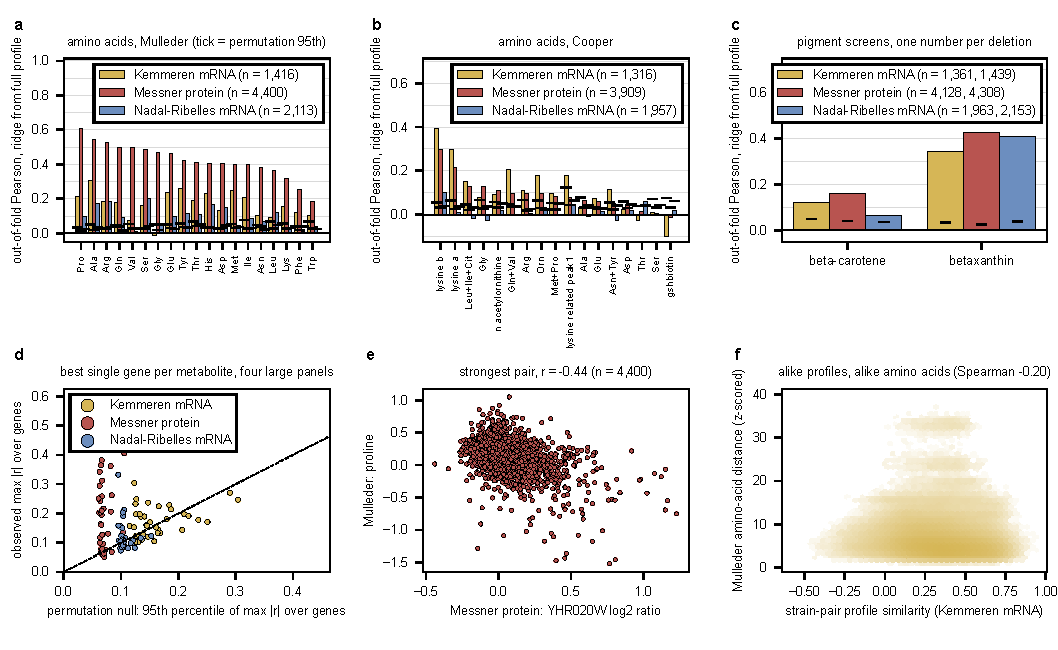
\includegraphics[width=\textwidth]{figures/expression_metabolic_yko_correlation.pdf}
\caption[]{\textbf{A deletion's proteome predicts its amino-acid pools at $0.4$ to $0.6$
out of fold, its transcriptome at $0.1$ to $0.3$, and every bar of the two large
amino-acid panels clears its permutation null.} \textbf{a}, \textbf{b}, out-of-fold
Pearson of a ridge from the whole profile to each amino acid (Mulleder, Cooper), one bar
per source, the black tick the permutation 95th percentile of the same statistic.
\textbf{c}, the two pigment screens. \textbf{d}, the largest single-feature $|r|$ per
metabolite against the permutation null of that maximum, for the four large panels; the
Kemmeren null is wide because the metabolite values are heavy tailed. \textbf{e}, the
strongest single pair, the prolyl-tRNA synthetase protein against the proline pool.
\textbf{f}, profile similarity of a strain pair against the amino-acid distance of the
same pair over 1.0 million Kemmeren pairs. Generated by
\file{expression_metabolic_yko_correlation.py}.}
\label{fig:reads}
\end{figure}

\subsection{The proteome carries the amino-acid pools; the transcriptome carries less of them\secstatus{todo}}
\label{sec:findings-amino}

On the 19 Mulleder amino acids the ridge from the Messner proteome reads a median
out-of-fold Pearson of $0.41$ over 4{,}400 shared deletions, every one of the 19 above
its permutation 95th percentile (which sits between $0.03$ and $0.08$); proline reads
$0.61$, alanine $0.55$, arginine $0.52$, glutamine $0.50$. The same ridge from the
Kemmeren transcriptome reads a median of $0.18$ over 1{,}416 shared deletions, 18 of 19
above null; alanine reads $0.31$, tyrosine $0.26$, methionine $0.25$
(\cref{tab:amino-acids}). Cooper 2010 repeats the ordering at lower strength, a median
of $0.08$ from protein and $0.10$ from mRNA, with the lysine peaks at $0.30$ to $0.39$;
its values are ratios to a plate mean from a single measurement, so its ceiling is
lower than Mulleder's before any source is asked to reach it.
\src{experiments/028-knockout-expression/results/expression_metabolic_yko_correlation.json}

%% SOURCE: tables/amino_acids.tex, generated by expression_metabolic_yko_correlation.py
%% GENERATED by experiments/028-knockout-expression/scripts/expression_metabolic_yko_correlation.py
%% from results/expression_metabolic_yko_correlation.json. Do not edit by hand.
%% SOURCE: results/expression_metabolic_yko_correlation.json via expression_metabolic_yko_correlation.py
\begin{table}[htbp]
  \centering
  \footnotesize
  \caption[The Mulleder amino acids by source]{The 19 Mulleder 2016 amino acids, ordered by the proteome's score. Ridge $r$ is the out-of-fold Pearson from the whole profile with the permutation 95th percentile in parentheses; the top gene is the single feature with the largest $|r|$ against the metabolite across the shared deletions, with its sign. \src{experiments/028-knockout-expression/scripts/expression_metabolic_yko_correlation.py}}
  \label{tab:amino-acids}
  \setlength{\tabcolsep}{3pt}
  \begin{tabular}{@{}lp{1.7cm}p{2.0cm}p{1.7cm}p{2.0cm}p{1.7cm}p{2.0cm}@{}}
    \toprule
    amino acid & Kemmeren mRNA ridge $r$ (null) & top gene & Messner protein ridge $r$ (null) & top gene & Nadal-Ribelles mRNA ridge $r$ (null) & top gene \\
    \midrule
    proline & $0.21$ (0.03) & \gene{RTG2} $+0.27$ & $0.61$ (0.02) & \file{YHR020W} $-0.44$ & $0.10$ (0.02) & \gene{COX4} $+0.10$ \\
    alanine & $0.31$ (0.05) & \gene{ALT2} $-0.22$ & $0.55$ (0.02) & \gene{ALT1} $+0.38$ & $0.18$ (0.03) & \gene{SOD1} $-0.19$ \\
    arginine & $0.18$ (0.03) & \file{YOR366W} $+0.16$ & $0.52$ (0.03) & \gene{TSL1} $-0.29$ & $0.19$ (0.04) & \gene{TSA1} $+0.16$ \\
    glutamine & $0.18$ (0.05) & \gene{RTG2} $+0.20$ & $0.50$ (0.04) & \gene{KRS1} $-0.41$ & $0.09$ (0.02) & \gene{SOD1} $+0.12$ \\
    valine & $0.07$ (0.05) & \gene{OCA1} $-0.18$ & $0.50$ (0.03) & \gene{ILV2} $+0.36$ & $0.01$ (0.02) & \gene{EFB1} $+0.08$ \\
    serine & $0.16$ (0.03) & \gene{DUR12} $-0.17$ & $0.48$ (0.03) & \gene{LEU4} $-0.37$ & $0.20$ (0.04) & \gene{SOD1} $+0.21$ \\
    glycine & $-0.01$ (0.05) & \gene{SRL4} $-0.11$ & $0.47$ (0.02) & \gene{SHM2} $+0.43$ & $0.05$ (0.05) & \gene{SOD1} $-0.10$ \\
    glutamate & $0.24$ (0.05) & \gene{RTG2} $+0.23$ & $0.46$ (0.03) & \file{YHR138C} $+0.26$ & $0.10$ (0.02) & \file{YGL188C} $+0.09$ \\
    tyrosine & $0.26$ (0.06) & \gene{GDH2} $+0.24$ & $0.42$ (0.04) & \gene{ARO4} $+0.34$ & $0.12$ (0.03) & \gene{SOD1} $-0.20$ \\
    threonine & $0.19$ (0.07) & \gene{YPS3} $-0.19$ & $0.41$ (0.04) & \gene{RNR4} $-0.20$ & $0.11$ (0.05) & \gene{TSA1} $-0.11$ \\
    histidine & $0.23$ (0.03) & \gene{RDL1} $-0.15$ & $0.40$ (0.04) & \gene{ATP4} $+0.20$ & $0.17$ (0.03) & \gene{TSA1} $+0.12$ \\
    aspartate & $0.13$ (0.02) & \gene{TOP1} $-0.15$ & $0.40$ (0.03) & \gene{DIC1} $+0.22$ & $0.15$ (0.05) & \gene{AHP1} $-0.16$ \\
    methionine & $0.25$ (0.05) & \gene{MCT1} $-0.25$ & $0.40$ (0.03) & \gene{ITR1} $+0.26$ & $0.05$ (0.04) & \gene{TPI1} $-0.12$ \\
    isoleucine & $0.21$ (0.08) & \gene{PDR12} $+0.17$ & $0.40$ (0.03) & \gene{GUA1} $+0.24$ & $0.08$ (0.03) & \gene{NPL4} $-0.11$ \\
    asparagine & $0.10$ (0.05) & \gene{CKA2} $+0.14$ & $0.38$ (0.04) & \gene{YHM2} $-0.21$ & $0.07$ (0.02) & \gene{TSA1} $-0.11$ \\
    leucine & $0.09$ (0.07) & \file{YPR059C} $+0.11$ & $0.36$ (0.03) & \gene{AAT2} $-0.31$ & $0.12$ (0.05) & \gene{SOD1} $+0.15$ \\
    lysine & $0.16$ (0.06) & \gene{RTG2} $+0.18$ & $0.32$ (0.03) & \gene{ARG56} $+0.16$ & $0.03$ (0.03) & \gene{ECM16} $-0.08$ \\
    phenylalanine & $0.12$ (0.04) & \gene{RTG2} $-0.16$ & $0.25$ (0.02) & \gene{TSL1} $-0.19$ & $0.01$ (0.04) & \gene{MSK1} $+0.08$ \\
    tryptophan & $0.10$ (0.07) & \file{YHL005C} $-0.13$ & $0.19$ (0.03) & \gene{ARG1} $+0.12$ & $0.04$ (0.03) & \gene{SHH4} $-0.09$ \\
    \bottomrule
  \end{tabular}
\end{table}


\notesec{The single features behind the strong reads are pathway enzymes} Proline's top
protein is the prolyl-tRNA synthetase \file{YHR020W} ($r = -0.44$ over 4{,}400
deletions), then \gene{ARO2} and \gene{THR1} at $-0.41$. Alanine's is \gene{ALT1}, the
alanine aminotransferase ($+0.38$), then \gene{ILV2} and \gene{SER1}. Glutamine's are
\gene{KRS1} ($-0.41$) and \gene{ARG7} ($-0.39$); arginine's are \gene{TSL1},
\gene{LSP1} and \gene{TPS2} at $-0.29$. From the transcriptome, alanine's top reporter
is \gene{ALT2} ($-0.22$), and the top reporter for proline, glutamine, glutamate, lysine
and phenylalanine is one gene, \gene{RTG2} of the retrograde response ($+0.16$ to
$+0.27$), the pathway that raises glutamate synthesis when mitochondrial function
falls. A strain whose proteome carries less of an amino acid's own
synthetase or transaminase carries more of the amino acid, which is the direction a
pool-and-flux picture predicts and not one a plate artifact would choose.

\subsection{The pigment screens read the same way\secstatus{todo}}
\label{sec:findings-pigment}

Betaxanthin, the Cachera 2023 titer proxy, reads $0.43$ from the proteome (4{,}308
shared deletions) and $0.35$ from the transcriptome (1{,}439), against nulls of $0.03$.
Its top proteins are \gene{COX13} ($-0.25$), \gene{DLD1} ($+0.22$) and \gene{ATP7}
($-0.22$), the respiratory signature the screen's own top hits carry. The Ozaydin 2013
beta-carotene colony score, an ordinal from $-5$ to $+5$ with 45\,\% of strains at zero,
reads $0.16$ from protein and $0.12$ from mRNA against nulls of $0.04$ to $0.05$, above
chance and far below the amino acids.
\src{experiments/028-knockout-expression/results/expression_metabolic_yko_correlation.json}

\subsection{Alike transcriptomes, alike amino-acid profiles\secstatus{todo}}
\label{sec:findings-structure}

Without choosing a metabolite: over the 1.0 million pairs of Kemmeren deletions, the
Spearman between profile similarity and amino-acid distance is $-0.196$ against a
permutation 95th percentile of $0.033$, and $-0.150$ on the 282 Cooper deletions with
every peak (null $0.077$). Strains whose transcriptomes look alike have amino-acid
pools that sit close together. From the proteome the same read is $-0.046$ on Mulleder
(9.7 million pairs, null $0.003$) and a null $+0.002$ on Cooper. So the proteome
predicts individual amino acids far better than the transcriptome, yet its whole-profile
similarity tracks the amino-acid profile less. Plausible mechanism, unverified: most
Messner deletions barely move the proteome, so pairwise profile Pearson among them is
noise, while the ridge reads the few proteins that do move.
\src{experiments/028-knockout-expression/results/expression_metabolic_yko_correlation.json}

\subsection{Nadal-Ribelles reads the phenotype through one program\secstatus{todo}}
\label{sec:findings-nadal}

The perturb-seq pseudobulk shares 2{,}113 deletions with Mulleder and reads a median
out-of-fold Pearson of $0.10$, 17 of 19 amino acids above nulls of $0.02$ to $0.05$;
serine reads $0.20$, arginine $0.19$, alanine $0.18$, histidine $0.17$, and
phenylalanine, valine, lysine and tryptophan read at chance. On Cooper it reads a
median of $0.01$ with 2 of 17 peaks above null, and on the beta-carotene score $0.07$
against a null of $0.04$. On betaxanthin it reads $0.41$ over 2{,}153 deletions, level
with the transcriptome's $0.35$ and the proteome's $0.43$. The structure read is
$-0.067$ on Mulleder (2.2 million pairs, null $0.034$) and $-0.059$ on Cooper, inside
its null of $0.076$.
\src{experiments/028-knockout-expression/results/expression_metabolic_yko_correlation.json}

\notesec{Every Nadal read runs through the same reporters} The top single features are
the same handful whichever metabolite is asked: \gene{TSA1}, \gene{SOD1}, \gene{AHP1},
\gene{GPX2} and \gene{TRR1} for betaxanthin ($-0.33$ to $-0.27$), and \gene{SOD1},
\gene{TSA1}, \gene{AHP1}, \gene{GRE2} for serine, arginine, histidine ($+0.11$ to
$+0.21$) and alanine ($-0.19$). These are the oxidative-stress reporters, one
transcriptional program. So what the atlas carries about the metabolic phenotype is the
position of each deletion on that axis; the amino acids it reads are the ones that axis
happens to track, and the ones it cannot read (phenylalanine, valine, lysine,
tryptophan) are the ones the proteome reads through their own enzymes. Plausible
mechanism, unverified: the oxidative-stress program is large enough to survive the
per-cell counting noise and the batch structure that erase the small, gene-specific
responses, which is why the atlas fails to replicate the compendium yet reads a
large-effect phenotype as well as the compendium does.

\notesec{What this says about quality control} Agreement with an earlier compendium
is one test of a readout and the metabolic phenotype is another, and the two can
disagree. Nadal-Ribelles fails the first (cross-batch $r$ of $0.04$, per-deletion
agreement with Messner of $0.01$) and passes the second on the phenotype that its one
program tracks. A readout with no agreement and no metabolic read would have no
defense; this one has a narrow defense, and its use is bounded by it: a model trained
on it can learn the stress axis and should not be expected to learn the rest.

\subsection{The small panels read null, as their size predicts\secstatus{todo}}
\label{sec:findings-small}

Zelezniak 2018 shares 93 deletions with Kemmeren and 88 with Messner; da Silveira 2014
shares 121 and 116. A ridge over thousands of features on under 125 samples reads a
median out-of-fold Pearson of $-0.05$ (Zelezniak) and $0.00$ to $0.04$ (da Silveira),
with the da Silveira lipids that clear their null (23 of 147 from mRNA, 34 of 147 from
protein) at the rate a 5\,\% threshold produces on its own. These panels say nothing
about the question either way.
\src{experiments/028-knockout-expression/results/expression_metabolic_yko_correlation.json}
